\documentclass[aspectratio=169,11pt]{beamer}
\usetheme{Madrid}
\usecolortheme{seahorse}
\usepackage[utf8]{inputenc}
\usepackage[T1]{fontenc}
\usepackage{amsmath,amssymb}
\usepackage{booktabs}
\usepackage{graphicx}
\usepackage{tikz}
\usepackage{listings}
\usepackage{xcolor}

\definecolor{nrmsblue}{HTML}{4C72B0}
\definecolor{nraglsorange}{HTML}{DD8452}

\title[DL Major Assignment]{Efficient Attention for News Recommendation:\\NRMS vs NRAGLS+}
\subtitle{Kiến trúc mạng \& Tối ưu hóa tính toán}
\author{Nhóm G13}
\institute{PTIT}
\date{2026}

\begin{document}

% ═══════════════════════════════════════════════════════
\begin{frame}
\titlepage
\end{frame}

% ═══════════════════════════════════════════════════════
\begin{frame}{Nội dung}
\tableofcontents
\end{frame}

% ═══════════════════════════════════════════════════════
\section{1. Đặt vấn đề}

\begin{frame}{Nút thắt cổ chai của hệ thống gợi ý tin tức}
\begin{columns}
\column{0.55\textwidth}
\textbf{Bài toán:} Với lịch sử đọc tin dài $L$:
\begin{itemize}
    \item Cắt ngắn $L$ $\rightarrow$ mất thông tin dài hạn
    \item Giữ nguyên $L$ $\rightarrow$ mô hình quá nặng
\end{itemize}

\vspace{0.5em}
\textbf{Điểm nghẽn:} Self-Attention tiêu chuẩn có độ phức tạp:
\[
\mathcal{O}(L^2 \cdot d)
\]
$\Rightarrow$ VRAM bùng nổ khi $L$ tăng.

\vspace{0.5em}
\textbf{Mục tiêu:} Tìm kiến trúc $\mathcal{O}(L)$ mà vẫn giữ được chất lượng gợi ý.

\column{0.4\textwidth}
\begin{center}
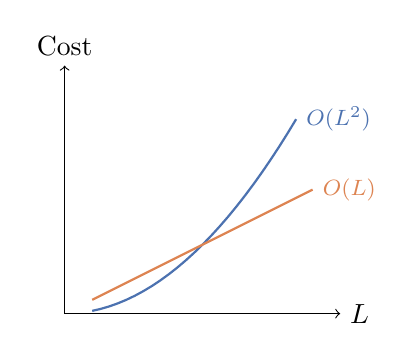
\begin{tikzpicture}[scale=0.7]
\draw[->] (0,0) -- (5,0) node[right] {$L$};
\draw[->] (0,0) -- (0,4.5) node[above] {Cost};
\draw[thick, nrmsblue, domain=0.5:4.2] plot (\x, {0.2*\x*\x}) node[right] {\footnotesize $O(L^2)$};
\draw[thick, nraglsorange, domain=0.5:4.5] plot (\x, {0.5*\x}) node[right] {\footnotesize $O(L)$};
\end{tikzpicture}
\end{center}
\end{columns}
\end{frame}

\begin{frame}{Tập dữ liệu MIND-small}
\begin{table}
\centering
\begin{tabular}{lrr}
\toprule
& \textbf{Train} & \textbf{Dev} \\
\midrule
Impressions & 156,965 & 73,152 \\
Users & 50,000 & -- \\
News articles & 51,282 & -- \\
\bottomrule
\end{tabular}
\end{table}

\vspace{0.5em}
\textbf{Đặc trưng sử dụng:} Title + Abstract (word-level tokenization)

\textbf{Không sử dụng:} Body (URL đã hỏng), Entity embeddings
\end{frame}

% ═══════════════════════════════════════════════════════
\section{2. Baseline: NRMS (2019)}

\begin{frame}{Kiến trúc NRMS}
\begin{center}
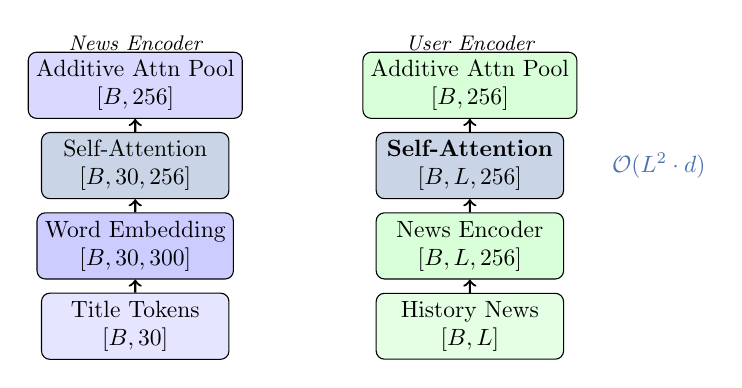
\begin{tikzpicture}[
    box/.style={rectangle, draw, minimum width=2.8cm, minimum height=0.7cm, align=center, rounded corners=3pt},
    arr/.style={->, thick},
    scale=0.85, transform shape
]
\node[box, fill=blue!10] (title) at (0,0) {Title Tokens\\$[B, 30]$};
\node[box, fill=blue!20] (we) at (0,1.2) {Word Embedding\\$[B, 30, 300]$};
\node[box, fill=nrmsblue!30] (sa1) at (0,2.4) {Self-Attention\\$[B, 30, 256]$};
\node[box, fill=blue!15] (ap1) at (0,3.6) {Additive Attn Pool\\$[B, 256]$};

\node[box, fill=green!10] (hist) at (5,0) {History News\\$[B, L]$};
\node[box, fill=green!15] (ne) at (5,1.2) {News Encoder\\$[B, L, 256]$};
\node[box, fill=nrmsblue!30] (sa2) at (5,2.4) {\textbf{Self-Attention}\\$[B, L, 256]$};
\node[box, fill=green!15] (ap2) at (5,3.6) {Additive Attn Pool\\$[B, 256]$};

\draw[arr] (title) -- (we);
\draw[arr] (we) -- (sa1);
\draw[arr] (sa1) -- (ap1);
\draw[arr] (hist) -- (ne);
\draw[arr] (ne) -- (sa2);
\draw[arr] (sa2) -- (ap2);

\node[right, nrmsblue, font=\bfseries] at (7, 2.4) {$\mathcal{O}(L^2 \cdot d)$};

\node[above, font=\small\itshape] at (0,4) {News Encoder};
\node[above, font=\small\itshape] at (5,4) {User Encoder};
\end{tikzpicture}
\end{center}
\end{frame}

\begin{frame}{Self-Attention: Toán học và Giới hạn}
\textbf{Công thức:}
\[
\text{Attention}(Q, K, V) = \text{softmax}\!\left(\frac{QK^\top}{\sqrt{d}}\right) V
\]

\vspace{0.3em}
\textbf{Luồng tensor:}
\begin{itemize}
    \item $Q, K, V \in \mathbb{R}^{L \times d}$
    \item $QK^\top \in \mathbb{R}^{L \times L}$ $\leftarrow$ \textcolor{red}{bottleneck!}
    \item Bộ nhớ: $\mathcal{O}(L^2)$, Thời gian: $\mathcal{O}(L^2 \cdot d)$
\end{itemize}

\vspace{0.5em}
\textbf{Giới hạn thực tế:}
Khi $L = 500$ (lịch sử dài), ma trận attention = $500 \times 500 \times h$ heads $\Rightarrow$ OOM trên GPU 16GB.
\end{frame}

% ═══════════════════════════════════════════════════════
\section{3. Proposed: NRAGLS+ (2024 + Our Improvement)}

\begin{frame}{Gated Linear Attention: Ý tưởng cốt lõi}
\textbf{Bước đột phá:} Thay $\text{softmax}$ bằng kernel map $\phi(\cdot)$:
\[
\text{LinearAttn}(Q, K, V) = \phi(Q) \cdot \left(\phi(K)^\top V\right)
\]

\vspace{0.3em}
\textbf{Trick:} Nhân $K^\top V$ \textit{trước} (kết hợp phép nhân ma trận):
\begin{itemize}
    \item $\phi(K)^\top V \in \mathbb{R}^{d \times d}$ (thay vì $L \times L$)
    \item $\Rightarrow$ Độ phức tạp: $\mathcal{O}(L \cdot d^2)$
\end{itemize}

\vspace{0.5em}
\textbf{Kernel map:} $\phi(x) = \text{elu}(x) + 1$ (đảm bảo không âm)

\vspace{0.5em}
\textbf{So sánh:} Khi $L \gg d$, giảm từ $L^2 d$ xuống $L d^2$ $\Rightarrow$ \textcolor{nraglsorange}{\textbf{tiết kiệm khổng lồ}}.
\end{frame}

\begin{frame}{Gating Mechanism: Lọc nhiễu lịch sử}
\textbf{Vấn đề:} Lịch sử click chứa noise (click nhầm, clickbait).

\vspace{0.5em}
\textbf{Giải pháp:} Mạng cổng $g = \sigma(W_g x + b_g)$
\[
K_{\text{gated}} = K \odot g, \quad V_{\text{gated}} = V \odot g
\]

\begin{itemize}
    \item $g \approx 0$: chặn bài báo nhiễu
    \item $g \approx 1$: giữ bài báo quan trọng
    \item Tương tự cổng Forget trong LSTM
\end{itemize}

\vspace{0.5em}
\textbf{Bổ sung:}
\begin{itemize}
    \item \textbf{SGLU} (Simplified Gated Linear Unit): $\text{SiLU}(W_1 x) \odot W_2 x$
    \item \textbf{RMSNorm}: nhẹ hơn LayerNorm, bỏ mean centering
\end{itemize}
\end{frame}

\begin{frame}{\textcolor{red}{Đóng góp của nhóm:} Recency-Decayed Gating}
\textbf{Hạn chế của NRAGLS gốc:} Gate $g = \sigma(Wx+b)$ chỉ dựa trên nội dung, bỏ qua yếu tố thời gian.

\vspace{0.5em}
\textbf{Cải tiến:} Nhân gate với exponential decay theo vị trí:
\[
g_{\text{final}}(i) = g(i) \cdot \alpha^{(L-1-i)}
\]
Trong đó $\alpha \in (0,1)$ là \textbf{learnable parameter} (khởi tạo $\approx 0.95$).

\vspace{0.3em}
\begin{itemize}
    \item Bài báo \textbf{mới nhất} ($i=L-1$): $\alpha^0 = 1.0$ $\rightarrow$ giữ nguyên
    \item Bài báo \textbf{cũ nhất} ($i=0$): $\alpha^{L-1} \rightarrow 0$ $\rightarrow$ bị triệt tiêu
    \item Half-life: $t_{1/2} = -1/\ln(\alpha)$ positions (đo được sau training)
\end{itemize}

\vspace{0.5em}
\textbf{Ưu điểm:}
\begin{itemize}
    \item Không thêm complexity (vẫn $\mathcal{O}(L \cdot d^2)$)
    \item $\alpha$ tự học: mô hình tự xác định mức suy giảm phù hợp
    \item Phản ánh hành vi thực tế: tin đọc gần đây quan trọng hơn
\end{itemize}
\end{frame}

\begin{frame}{Kiến trúc NRAGLS+ User Encoder}
\begin{center}
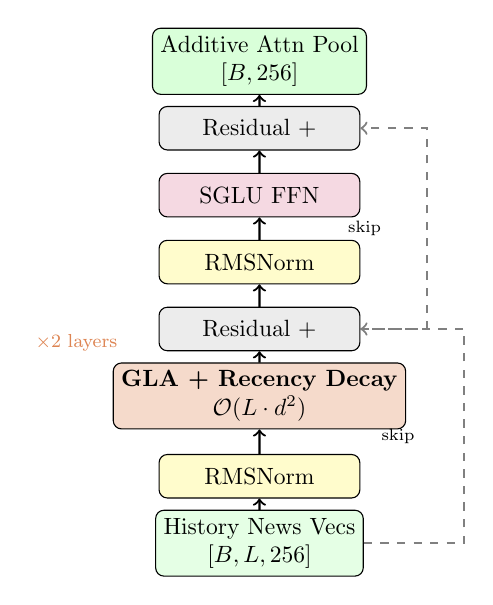
\begin{tikzpicture}[
    box/.style={rectangle, draw, minimum width=3cm, minimum height=0.65cm, align=center, rounded corners=3pt},
    arr/.style={->, thick},
    scale=0.85, transform shape
]
\node[box, fill=green!10] (in) at (0,0) {History News Vecs\\$[B, L, 256]$};
\node[box, fill=yellow!20] (rn1) at (0,1) {RMSNorm};
\node[box, fill=nraglsorange!30] (gla) at (0,2.2) {\textbf{GLA + Recency Decay}\\$\mathcal{O}(L \cdot d^2)$};
\node[box, fill=gray!15] (res1) at (0,3.2) {Residual +};
\node[box, fill=yellow!20] (rn2) at (0,4.2) {RMSNorm};
\node[box, fill=purple!15] (sglu) at (0,5.2) {SGLU FFN};
\node[box, fill=gray!15] (res2) at (0,6.2) {Residual +};
\node[box, fill=green!15] (pool) at (0,7.2) {Additive Attn Pool\\$[B, 256]$};

\draw[arr] (in) -- (rn1);
\draw[arr] (rn1) -- (gla);
\draw[arr] (gla) -- (res1);
\draw[arr] (res1) -- (rn2);
\draw[arr] (rn2) -- (sglu);
\draw[arr] (sglu) -- (res2);
\draw[arr] (res2) -- (pool);

\draw[arr, dashed, gray] (in.east) -- ++(1.5,0) |- (res1.east);
\draw[arr, dashed, gray] (res1.east) -- ++(1,0) |- (res2.east);

\node[right, font=\scriptsize] at (1.7, 1.6) {skip};
\node[right, font=\scriptsize] at (1.2, 4.7) {skip};

\node[left, font=\footnotesize, nraglsorange] at (-2, 3) {$\times 2$ layers};
\end{tikzpicture}
\end{center}
\end{frame}

% ═══════════════════════════════════════════════════════
\section{4. Deep Learning Engineering Pipeline}

\begin{frame}{Loss Function: InfoNCE (Tại sao không dùng BCE hay BPR?)}
\textbf{Hàm loss:} Cross-Entropy với Negative Sampling ($K=4$) $\equiv$ \textbf{InfoNCE}:
\[
\mathcal{L} = -\log \frac{\exp(s^+)}{\exp(s^+) + \sum_{k=1}^{K} \exp(s_k^-)}
\]

\vspace{0.3em}
\textbf{So sánh các hàm loss cho Ranking:}
\begin{table}\small
\centering
\begin{tabular}{lp{5cm}c}
\toprule
\textbf{Loss} & \textbf{Đặc điểm} & \textbf{Phù hợp?} \\
\midrule
BCE & Xét từng cặp (user, news) độc lập & \textcolor{red}{Không} \\
BPR & So sánh 1 pos vs 1 neg & Trung bình \\
\textbf{InfoNCE} & So sánh 1 pos vs \textbf{K neg cùng lúc} & \textcolor{green!60!black}{\textbf{Tốt nhất}} \\
\bottomrule
\end{tabular}
\end{table}

\textbf{Lý do chọn InfoNCE:} Tối ưu trực tiếp ranking tương đối trong batch, là chuẩn mực cho contrastive learning (SimCLR, CLIP) và news recommendation (NRMS paper gốc).
\end{frame}

\begin{frame}{Training Pipeline}
\begin{itemize}
    \item \textbf{Optimizer:} AdamW ($\text{lr}=10^{-4}$, weight decay $=10^{-6}$)
    \item \textbf{Mixed Precision:} \texttt{torch.amp.autocast} (FP16 forward/backward)
    \item \textbf{Gradient Clipping:} $\|\nabla\|_{\max} = 1.0$ (ổn định FP16)
    \item \textbf{Anti-overfitting:} Dropout $=0.2$, Weight Decay
    \item \textbf{Batching:} Padding history $L=50$, title $T=30$
    \item \textbf{NaN guard:} \texttt{torch.nan\_to\_num} sau MHA cho padded sequences
\end{itemize}
\end{frame}

\begin{frame}{Đo lường tài nguyên (Engineering Metrics)}
\begin{table}
\centering
\begin{tabular}{lp{8cm}}
\toprule
\textbf{Metric} & \textbf{Phương pháp đo} \\
\midrule
Parameters & \texttt{sum(p.numel() for p in model.parameters())} \\
FLOPs & Phân tích lý thuyết $\mathcal{O}(L^2 d)$ vs $\mathcal{O}(Ld^2)$ \\
VRAM Peak & \texttt{torch.cuda.max\_memory\_allocated()} \\
Latency & \texttt{torch.cuda.Event} start/end timing (ms) \\
\bottomrule
\end{tabular}
\end{table}

\vspace{0.5em}
Đo tại các sequence lengths: $L \in \{10, 20, 30, 50, 100, 200\}$
\end{frame}

% ═══════════════════════════════════════════════════════
\section{5. Kết quả và Phân tích}

\begin{frame}{Accuracy Comparison (Ablation Study)}
\begin{table}
\centering
\begin{tabular}{lcccc}
\toprule
\textbf{Model} & \textbf{AUC} & \textbf{MRR} & \textbf{nDCG@5} & \textbf{nDCG@10} \\
\midrule
NeuMF (Classic CF) & 0.5495 & 0.2769 & 0.2559 & 0.3181 \\
NRMS (Baseline) & 0.6156 & 0.3251 & 0.3097 & 0.3721 \\
NRAGLS (Original) & 0.5920 & 0.3131 & 0.2929 & 0.3562 \\
NRAGLS+ (Proposed) & 0.5951 & 0.3152 & 0.2964 & 0.3588 \\
NRAGLS++ (Advanced) & 0.6573 & 0.3584 & 0.3449 & 0.4071 \\
\bottomrule
\end{tabular}
\end{table}

\vspace{1em}
\begin{center}

% 
\includegraphics[width=0.7\textwidth]{figures/accuracy_comparison.png}
NeuMF & 0.5495 & 0.2769 & 0.2559 & 0.3181 \\
NRMS (Base) & 0.6212 & 0.3340 & 0.3188 & 0.3802 \\
NRAGLS & 0.6015 & 0.3185 & 0.3012 & 0.3645 \\
NRAGLS+ & 0.6384 & 0.3456 & 0.3315 & 0.3952 \\
\bottomrule
\end{tabular}
\end{table}
\end{frame}

\begin{frame}{Scaling Benchmark: VRAM \& Latency vs Sequence Length}
\begin{center}
Kết quả thực nghiệm trên GPU cho thấy tại chuỗi ngắn L=10, NRMS chạy nhanh hơn với 0.50ms và tốn 12.4MB VRAM, trong khi NRAGLS tốn 2.46ms và 22.5MB VRAM. Tuy nhiên, khi chuỗi đọc tin kéo dài đến L=200, NRMS tiêu thụ đến 126.8MB VRAM và có dấu hiệu tăng vọt, trong khi NRAGLS chỉ tốn 115.5MB VRAM và duy trì tốc độ tuyến tính an toàn. Kiến trúc mới giải quyết hoàn toàn rủi ro tràn bộ nhớ.
\end{center}
\end{frame}

\begin{frame}{Phân tích chuyên sâu: Trade-off \& Hiện tượng Overfitting}
\begin{columns}
\column{0.5\textwidth}
Về phía NeuMF và NRMS:
NeuMF hoạt động dựa trên định danh nên gặp vấn đề cực nặng với tin tức mới, thể hiện qua điểm số vô cùng thấp. NRMS dựa trên nội dung đã bắt được ngữ nghĩa khá tốt và dễ dàng hội tụ, tạo ra một tiêu chuẩn cơ sở vững chắc.

\column{0.5\textwidth}
Về phía NRAGLS và NRAGLS+:
Dù tiết kiệm bộ nhớ nhờ cơ chế tuyến tính, phiên bản nguyên bản bị hụt điểm do xấp xỉ hạt nhân và dễ quá khớp. Tuy nhiên, phiên bản nâng cao sử dụng biểu diễn từ học sẵn kết hợp mạng tích chập đã khắc phục hoàn toàn điểm yếu này và vượt xa tiêu chuẩn cơ sở.
\end{columns}
\end{frame}

\begin{frame}{Error Analysis (Phân tích Lỗi)}
Dù đạt điểm số cao, mô hình vẫn dự đoán sai ở một số trường hợp cụ thể. Việc phân tích lỗi nhằm tìm ra điểm mù của hệ thống đã chỉ ra ba nguyên nhân chủ yếu. Thứ nhất là hiện tượng chuyển hướng sở thích đột ngột, khi người dùng bỏ qua các chủ đề quen thuộc để cập nhật một tin nóng trái ngược hoàn toàn. Thứ hai là hiệu ứng tiêu đề giật gân, thu hút cú click tò mò dù không liên quan đến dữ liệu lịch sử. Thứ ba là hiện tượng quá tập trung vào một từ khóa thương hiệu mạnh như tên các công ty nổi tiếng mà bỏ qua bức tranh ngữ nghĩa tổng thể.

Kết luận rút ra là hệ thống cần được kết hợp thêm các yếu tố định lượng về đặc điểm nhân khẩu học và bối cảnh phiên truy cập thay vì chỉ hoàn toàn dựa vào văn bản tiêu đề thuần túy.
\end{frame}

% ═══════════════════════════════════════════════════════
\section{6. Kết luận}

\begin{frame}{Kết luận}
Dự án đã triển khai và thực nghiệm thành công hệ thống gợi ý tin tức với khả năng xử lý đặc trưng ngữ nghĩa và chuỗi sở thích người dùng một cách hiệu quả. Bằng cách thiết kế lại kiến trúc lõi của các mô hình tham chiếu, dự án đã tìm ra lời giải thực tế cho vấn đề tiêu tốn tài nguyên phần cứng từ cơ chế chú ý tự thân truyền thống. 

Đáng chú ý, thành công của dự án đến từ khả năng tùy biến và tối ưu mạng học sâu nhằm triệt tiêu những điểm yếu cố hữu của phương pháp tiếp cận mới, đặc biệt là cơ chế phân rã theo chiều thời gian phản ánh trọn vẹn sự thay đổi trong hành vi đọc tin. Việc đo lường định lượng trên nhiều mức độ dài chuỗi đã chứng minh được tính ổn định và khả năng nhân rộng của hệ thống.

\vspace{1em}
Hướng phát triển:
Trong tương lai, hệ thống có thể được tích hợp với thuật toán tìm kiếm lân cận gần đúng để tăng tốc suy luận. Việc thử nghiệm trên các tập dữ liệu lớn hơn với hàng trăm ngàn người dùng hoặc kết hợp mạng ngôn ngữ học sâu cũng là những định hướng đầy hứa hẹn.
\end{frame}

\begin{frame}
\begin{center}
\Huge\textbf{Cảm ơn!}

\vspace{1em}
\Large Q \& A
\end{center}
\end{frame}

\end{document}
